The last category of approaches to solve TSP are \emph{Metaheuristics} we're
going to present, high-level and complex procedures that are powerful enough to
reach near-optimum solutions in a reasonable amount of time, even with huge
instances. Considering the NP-hardness of TSP, this is our best shot so far, if
we're satisfied with an approximate solution. Internally they uses the
precedent heuristics we presented: they're placed at the implementation level
considering the high-level formulation of metaheuristics.\\ Among all the
approaches presented during the years, we're going to introduce three of them that
works nicely on TSP.

\section{Variable Neighborhood Search}
\emph{Variable Neighborhood Search} (VNS) is a metaheuristic technique proposed in
1997 \citep{mladenovic1997variable}. When an algorithm explores a solution space
not using mathematical programming the final result may be very influenced by
the starting solution. Sometimes allowing the algorithm only to improve the
solution can stuck it in local minimum that can be way worse than the optimal
solution. So VNS consents the current solution to move in a random way to
give it a chance to escape from these points of minimum.\\

\begin{algorithm}[H]
\SetAlgoLined
\KwResult{An approximated solution}
    $x\ \leftarrow$ initial solution\;
    \While{time limit is not reached \emph{or} $k \le k_{max}$}{
        $x'\ \leftarrow\ shake(x, k)$\;
	    $x' \leftarrow\ localopt(x')$\;
        \eIf{$cost(x') \le cost(x)$}{$x \leftarrow x'$\;}{$k \leftarrow k+1$\;}
    }
    \caption{VNS}
\end{algorithm}

So, the procedure of VNS needs two fundamental element: the method that
improves the solution and the one that can disturb it to escape from possible
local minimum. The \emph{shaking} function that disturbs the solution usually
depends on a input value $k$ that defines the neighborhood size Then the local
search function finds a local minimum. If this new solution is better then the
one before it becomes the incumbent, otherwise the neighborhood size increases
by one. If the max neighborhood size is reached the algorithm stops.

\subsection{Implementation details}
In our implementation of VNS we adapt the possibility to start from a random
solution or from a precomputed one. More on this choice in the next section,
since we're going to face similar choices. In TSP terms the shake operation is
called \emph{kick}, as it is slightly modifies the incumbent by rearranging $k$
arcs. The procedure clearly has to modify the solution into a feasible on, the
implemented procedure has to be subtour-free. The new candidate solution is then
modified using $2$-opt moves refinement presented is the previous chapter since,
as claimed, for an interesting number of nodes, there's no point of using
$k$-opt moves, with $k \ge 3$.\\ 
Every time a better solution is found the incumbent is updated and VNS is reset
with starting $k$ value equals to some minimum, 3 in our implementation. In the
case that the local search did not produce a new optimum the neighborhood is
enlarged by increasing $k$, until $k$ reaches $k_{max}$, where the algorithms
terminates. The increment of $k$ as well as $k_{max}$ should be tuned according
to the time limit, since it's not optimal to waste time on small $k$ with no
improvements or waste possibilities by truncating the computation due to small
$k_{max}$.\\
This can be seen as a multi-start procedure as the one presented above, but with
a kicked solution instead of a total different one.


\section{Tabu Search}
\emph{Tabu Search}, among with VNS, is another important metaheuristic proposed
by Fred Glover in 1986\citep{glover1986future} and, as VNS, is based on
refinements.\\ Starting from a solution, one is willing to improve it with
refinements until a local optimum is reached (\emph{downhill}). From there, one
could restart from another initial solution (multi-start) or restart from a
similar one by shaking it. Instead of those solutions, it's possible to insist
on the refinement subroutine and apply the refinement anyway. Since the solution
is stuck in a local optimum, the refinement will not improve the solution (it's
not a refinement at all!) but it will worse it. The idea is to apply as many
worsening move as possible until our subroutine produces a refinement that will
improve the solution (\emph{climbing}). At the end of this procedure, the
solution will be slightly different from the one stuck in the local optimum,
allowing us to restart from it in the refinement process.\\ To do so, an
important consideration has to be made: after the application of a worsening
move, the refinement subroutine will return a better solution by simply reverse
the move just done. For this reason, in the climbing part, it's important to
mark those moves as \emph{tabu}, forbidden moves that the refinement subroutine
will have to skip to produce a different starting solution.\\

\begin{algorithm}[H]
\SetAlgoLined
\KwResult{An approximated solution}
    $x\ \leftarrow$ initial solution\;
    \While{time limit is not reached}{
        $m\ \leftarrow\ move(x)$\;
        \If{$m$ is not tabu}{
            \If{$m$ is worsening move}{
                add $m$ to \emph{tabu list}
            }
            $x'\ \leftarrow\ apply\_move(x, m)$\;
        }
    }
    \caption{Tabu Search}
\end{algorithm}

Applied to TSP case, the refinement subroutine is $2$-opt move and the move is
the rearranging of 2 arcs. Initially, we will apply as many moves as possible in
order to improve the solution (\emph{downhill}). We can notice those moves by the
analysis of the $\Delta$ returned by the procedure: if $\Delta < 0$, it's an
improving move, otherwise it's a worsening one. After being stuck in a local
optimum, we can apply moves with $\Delta > 0$ until an improving one can be
found (\emph{climbing}) while marking all the nodes involved in the moves as
\emph{tabu nodes}. This is a simplification since we should declare the arcs
tabu (caused they're better representative of the move). Those nodes will be
stored in a \emph{tabu list} available to the $2$-opt move algorithm in order to
avoid them. We missed an important detail while defining the tabu moves: after
many iterations, almost every nodes will be marked as tabu. For that reason, we
have to release those nodes after some time, usually fixed, called
\emph{tenure}, which defines the maximum size of the tabu list. 

\subsection{Implementation details}
An initial solution has to be selected and, as in VNS, one could simply take it
randomly. A huge problem arise, because the first downhill could occupy the
majority of the time limit. $2$-opt moves are certain fast but still costly. To
explain this, let's analyze how $\Delta$ changes during iterations.

\begin{claim}
    Using GRASP as initial solution drastically improves the computation time on
    the first downhill.
\end{claim}

\begin{figure}[h!]
    \centering
    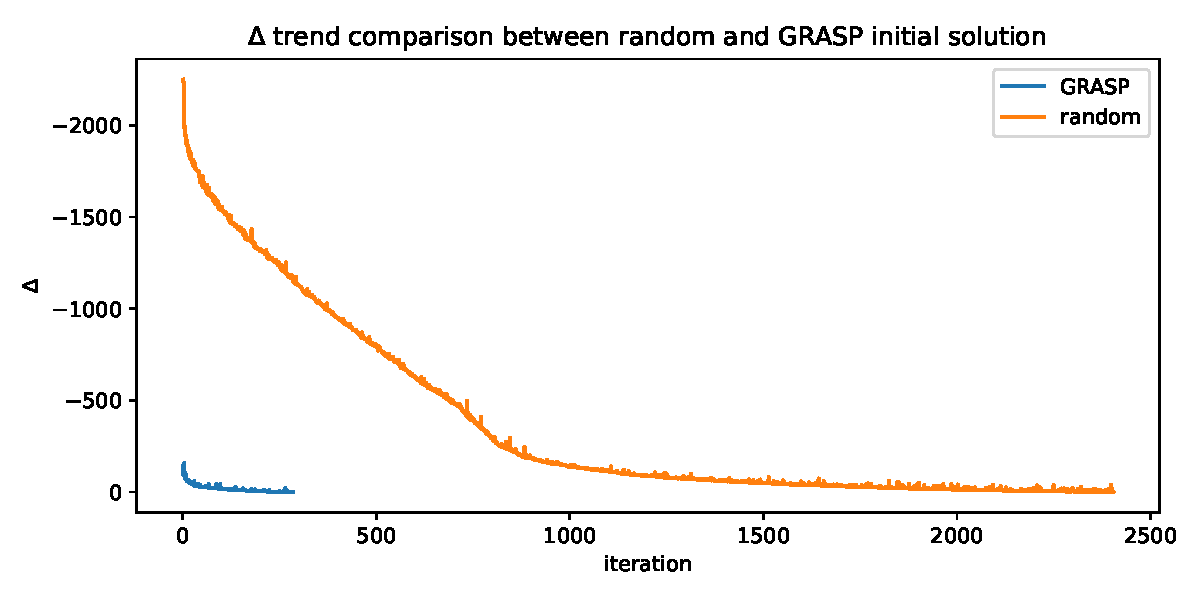
\includegraphics[width=0.78\textwidth]{figures/delta_trend}
    \caption[$\Delta$ trend for different initial solution]{\centering $\Delta$ trend for
    different initial solution. Notice that it's not monotonic}
\end{figure}

This represent the typical trend of $\Delta$ for an instance centered in a 1000
x 1000 box (that explain $\Delta$ in absolute values) for the first downhill.
Future downhills and climbings are similar in the sense that both of them
occupies just few iterations each. Using a GRASP as feeder for an initial
solution (blue line), it's rare to encounter costly crossing (initials are
typically $\sim-100$) and $\Delta$ drops very quickly ($\Delta < 1$ in $\sim250$
iterations). For a random start the situation is different (orange line):
initial $\Delta$ could be very high and there's a typical linear drop followed
by a logarithmic one until no more moves are possible. This typically takes 10
times the iterations using GRAPS as initial solution. For that reason, we will
feed the algorithms using the best GRASP solution among 500 starts, so more time
will be spent on the object in analysis: metaheuristic.\\ One could reply by
saying that our future analysis will be bias against GRASP-ish solutions. Well,
we can't really argue against that, only partially. One could assert that among
the near-optimal solutions, GRAPS don't produces the best ones, even if refined.
We have to remind that refinement could change lot of tour structure and, in
general, don't produce the optimal one, just a very good one. So there is no way
to think that a initially random-refined solution will be better than a
GRAPS-refined one. This justifies the choice of GRAPS among all the constructive
heuristics presented when dealing this kind of situations.\\ 
Another possible degree of freedom in Tabu Search implementation lies in the
tabu list. We keep the things as simple as possible, by tracking the iteration
number when the nodes were marked as tabu and compare it with the actual one: if
the difference is less than the tenure, the nodes is still tabu. There's no need
to implement an actual list, just an array of time stamps.\\
The last point is how to deal the neighborhood size while searching for
solutions. In this case the tenure play the same role as the kick strength in
VNS: by letting it change it's possible to define two phases:
\emph{intensification} and \emph{diversification}. In the first one the tenure is
kept high and lots of nodes will be marked as tabu: there's a small degree of
freedom and new solution will be very similar to the actual one. In the second
one, in which the tenure is small, few nodes will be blocked and there's the
possibility to find very different solutions. A switch between this two phases
is beneficial. The tenure values as well as the phases length are chosen
according to the number of nodes for the first one and according to the time
limit for the second one: we let switch between the phases around two/three
dozen of times during computation.

\section{Genetic algorithm}
The \emph{genetic algorithm} is one of the most popular metaheuristic
techniques. It is widely used in operation research and optimization problem
and it inspired by the natural selection. The idea behind the algorithm exploit
the possibility to merge two different elements of a population to create a new
one that hopefully combines the best characteristic of both parents generating
a better element. For this purpose, when a problem is defined, it is necessary
to establish a measure of performance that in our case is intrinsic considering
we are dealing with an optimization problem. 

The process usually follows the same steps. First of all, a population of $n$
candidate solutions to the problem is generated with a significant randomness
component since diversity is a fundamental feature. Then, a percentage of these
candidates is paired: they returns a new child solution from each pair combining
their chromosome, a data structure containing main information of the solution.
These children are inserted in the population and now among all the candidate
solutions some of them are discarded (\emph{killed}) to keep the population
constant. This series of operations are performed in what is called
\emph{epoch}.\\
By applying a random killing process and a random children procedure there's no
reason to think that the population will improve in terms of cost or, to be
more precise, in term of \emph{fitness}, which is defined as the capacity to
adapt to the environment. Anyway, in our context is simply the cost of a
solution, but this can be adapted to take into account additional constraints.
For this reason, some killing strategies will be discusses and, in addition to
this, \emph{mutations} will be added after children generation: random
improvement of certain solutions. For evolutionary reasons, the best candidate
among epochs, the \emph{champion}, will see its cost decrease, and it will be
returned after the process.

\begin{algorithm}[H]
\SetAlgoLined
\KwResult{An approximated solution}
    \emph{population} $\leftarrow$ n random solutions\;
    \While{time limit is not reached}{
        sample 2k \emph{parent} solution from \emph{population}\;
        \ForEach{pair p} {
            \emph{population} $\leftarrow$ add p \emph{child}\;
        }
        \emph{population} $\leftarrow$ mutate(population)\;
        \emph{population} $\leftarrow$ kill(population)\;
    }
    \emph{sol} $\leftarrow$ best candidate in \emph{population}
    \caption{Genetic Algorithm}
\end{algorithm}

\subsection{Implementation details}
In genetic algorithms implementation choices are mostly based on how solutions
are randomly generated, how they are map into a chromosome and how chromosomes
are combined. In case of TSP the most straightforward way to represent a
solution is an array of length $n$ nodes representing the order in which nodes
are visited. Those instances are created as a random permutation of the nodes.
Anyway, we decided to include very few GRASP solution (generated after just one
start, so they can be not so good). In our tests this speed-up the process
especially in initial epochs.\\
To combine two chromosome they are both split in left and right part. Child left
part is the same of parent 1. Then, all the unvisited nodes of the right part of
parent 2 by the child are added. In this way the child could not visit all the
nodes: the child generation procedure ends with an application of extra-mileage
algorithm to complete the solution and since it's a $\mathcal{O}(n^3)$
operation, this could drive the performances of the whole metaheuristics. In
fact, even if in our tests in the majority of cases only few nodes are left to
visit, in some cases that number could grow to $\sim\nicefrac{3}{8}$ of the total
number of nodes, and that could be costly. One normally should include a
refinement procedure to the child generated, but we decided to skip this
process. As we seen in Tabu Search section, the application of a complete
$2$-opt refinement to a random (or near-random) instance could be costly: we
decided to perform more epochs instead of spending time on this.\\
The mutation procedure is performed using $2$-opt moves on a certain number of
elements of the population. To balance the cost of the operation, we decided to
apply just very few moves to lots of members ($\sim$ 30\% of total population):
in this way we improve a lot the average fitness because, as we show in $\Delta$
trend graph, just few moves applied to a random solution are sufficient: we
decided to apply few dozen of $2$-opt moves, that corresponds to the $\Delta$
before the linear part of the trend.\\
The killing process is not random. One could be tempted to kill the worse
solutions, but they are still useful because they could act as a kick (in VNS
terms), so they could provide interesting and beneficial sub paths for the entire
population. Instead of that, one could analyze the fitness of the population and
do some statistics about that. Our implementation is simpler: we just keep away
from killing process some of the best solution ($\sim$ 20\% of total
population), among the rest of the population
the solutions to be killed are taken at random.\\
To improve even more the best champion found among epochs, we decided to spent some final
time by performing $2$-opt refinements on it.

\section{Metaheuristics comparison}
In this last section we're going to test the three metaheuristics presented,
including the $2$-opt multi start since it's a nice competitor of those. We
tested against 20 instances of 2000 nodes. We tested the
objective as well as how fast they reach it.

Genetic algorithm performances are quite variable, in the sense that certain
runs are comparable with the others metaheuristic, and in some other it cannot
reach good results. This is clear due to the randomness present in each step of
the process. The parameters tuning is performed to try to avoid this kind of
variabilities, but seems unavoidable, at least when the time limit is too low to
let the population reach good average fitness. Anyway, genetic algorithm can be
competitive in other scenario that we will present later on.\\
For this reason, while analyzing the objective reached at the end of the
process, let's exclude for a moment genetic algorithm.

\begin{claim}
    While genetic algorithm's variability makes him not competitive in terms of
    objective, $2$-opt multi start and tabu search are the best ones (even the
    last is more robust), followed by VNS.
\end{claim}

\newpage
\begin{figure}[h!]
    \centering
        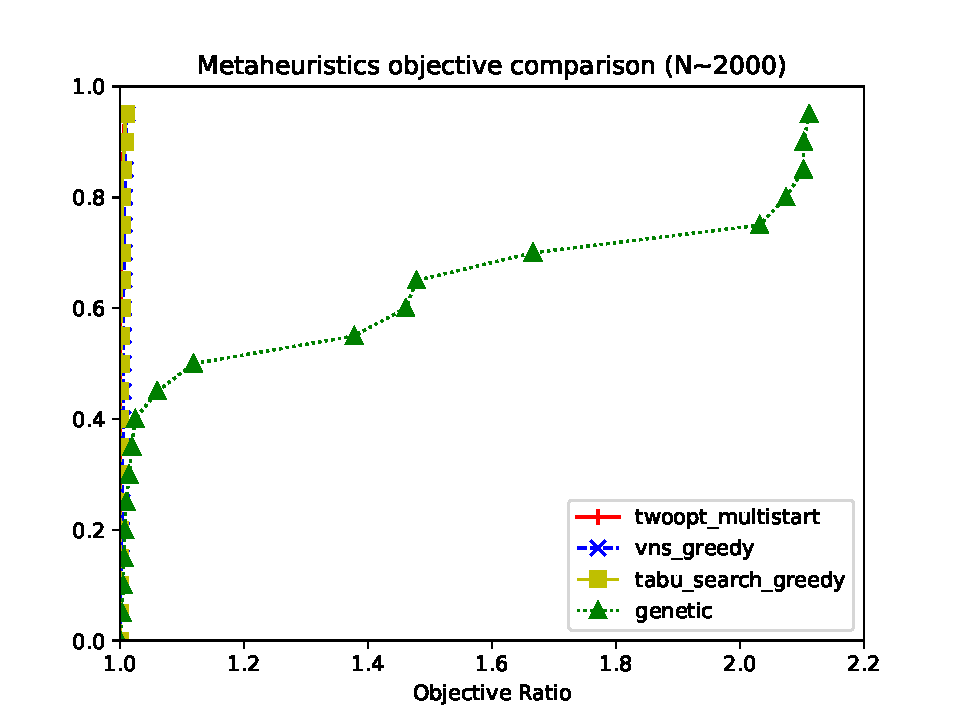
\includegraphics[width=0.8\linewidth]{figures/meta_results.pdf}
        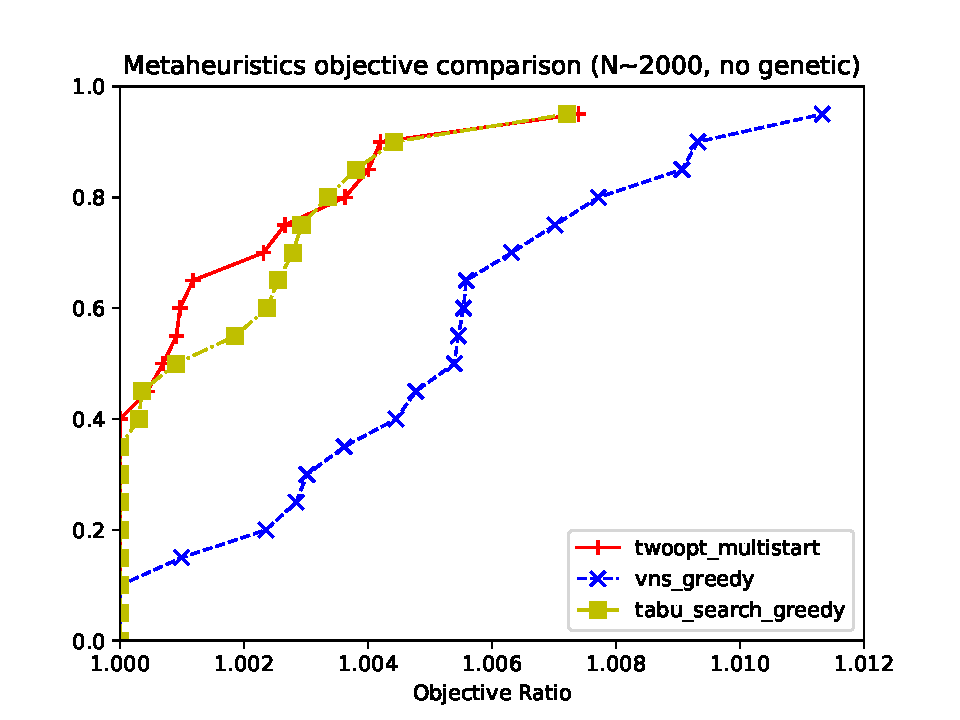
\includegraphics[width=0.8\linewidth]{figures/meta_results_wogenetic.pdf}
        \caption[Metaheuristics objective comparison]{Metaheuristics objective comparison (bottom: genetic algorithm excluded)}
\end{figure}


All of the left three approaches are quite good (the ratio on bottom graph is
pretty low) but a none of those reached $<3\%$ from the exact solution. VNS seems the
third best one, while both Tabu Search and $2$-opt multi start seems the best
options so far. In the case of $2$-opt multi start, that achieves slightly better
results compared with Tabu Search, the multi start approach helps a lot but on
this we noticed some variability that is not present in Tabu Search, that looks
like more robust since it works on an single initial solution: in low time limit
scenario, that would be our choice if one wouldn't take the risk to bet, even if
on average works pretty well.\\

For the last comparison, we solved to optimality the same instances and computed
the exact moment when the objective reached 5\%, 10\%, 50\% from the optimal
solution. This one is a comparison between times that makes possible to analyze
the speed over convergence.\\

\begin{claim}
    Overall, Tabu Search is the fastest algorithm to reaches low
    percentages from optimality. VNS is the second best choice but only if we
    restrict on higher percentages: it slow to achieve near-optimal
    solutions. $2$-opt multi start and genetic algorithm are competitive only at
    low percentages.
\end{claim}

\begin{figure}[h]
    \centering
    \begin{minipage}{.50\textwidth}
        \centering
        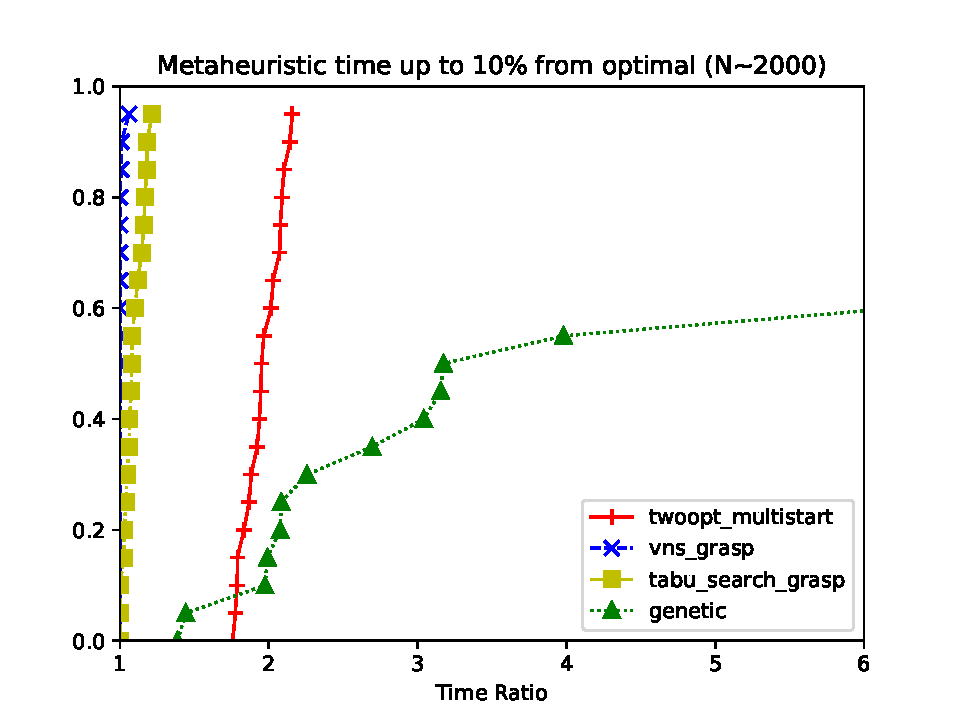
\includegraphics[width=\linewidth]{figures/meta_10.pdf}
    \end{minipage}%
    \begin{minipage}{.50\textwidth}
        \centering
        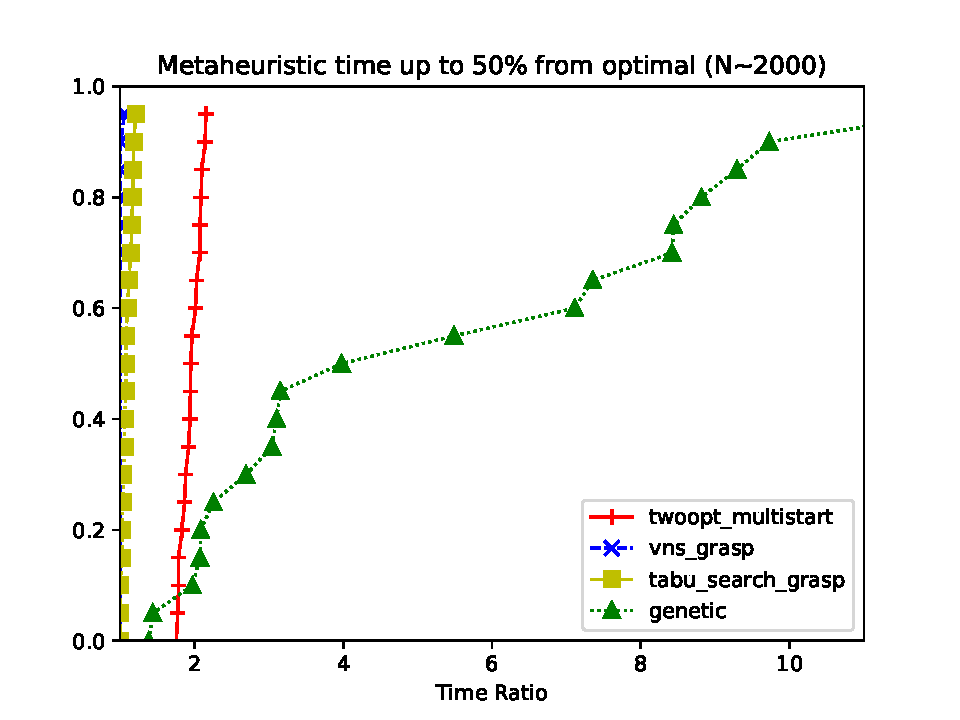
\includegraphics[width=\linewidth]{figures/meta_50.pdf}
    \end{minipage}
    \caption[Metaheuristics time to 10\% and 50\% from optimality
    comparison]{\centering Metaheuristics time to 10\% (left) and 50\% (right) from optimality
    comparison}
\end{figure}


\begin{figure}[h]
    \centering
        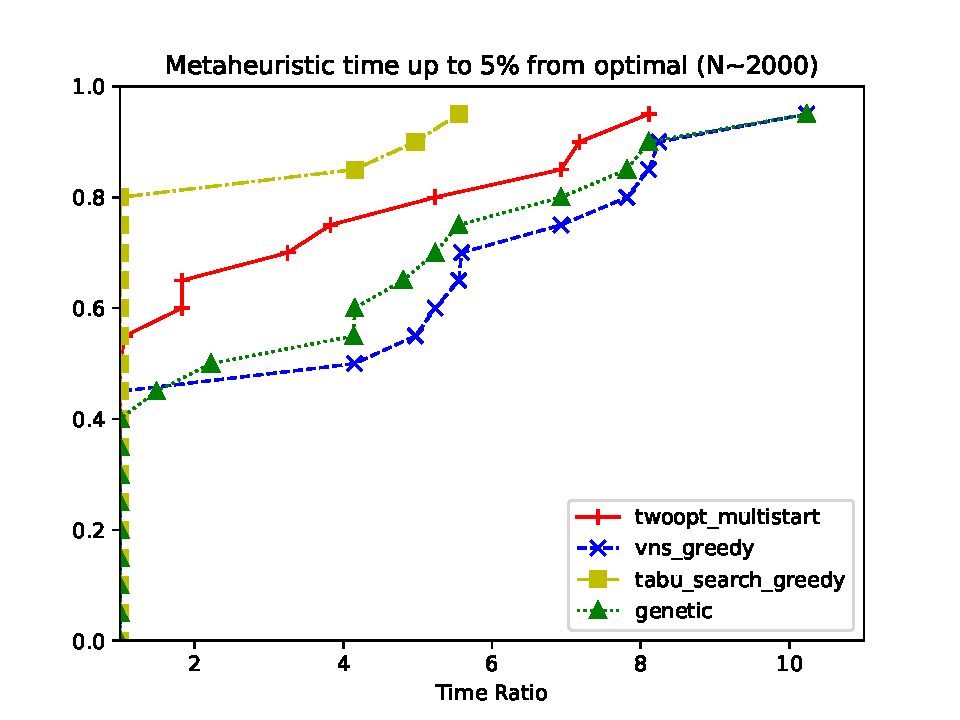
\includegraphics[width=0.75\linewidth]{figures/meta_5.pdf}
    \caption{\centering Metaheuristics time to 5\% from optimality
    comparison}
\end{figure}

Tabu Search is the winner of this round, it's fast to achieve both near-optimal
and more distant solution.\\

We have to state that the analysis of 10\% and 50\% are biased against the
initial starting solution obtained with GRASP in both Tabu Search, VNS and
$2$-opt that share the same analysis in those cases. We can observe that a
initial GRAPS-refined solution is not enough to obtain 50\% from optimal: in
those case, on average, the trend of the three methods should be exactly the
same because the first downhill should be  the same. Let's now suppose that both
shares the first downhill as well as the first local optimum and that a <50\%
solution can be obtained as the second local optimum encountered. Based on the
trends we observed during all the tests done we're now trying to guess the three
behaviours: \begin{itemize}
    \item $2$-opt multi start: after a shared first downhill, an $\epsilon$-cost
        restart is preformed followed by longer, and costly, downhills (and
        restarts) until the second local optimum
    \item VNS: after a shared first downhill, an $\epsilon$-cost
        \say{restart} is preformed by a kick, that move the solution near the
        last one, followed by a shorter downhills (and kicks) until the second
        local optimum
    \item Tabu Search: after a shared first downhill, very short climbing and
        downhills will follows until the second local optimum
\end{itemize}
For reaching 10\% and 50\% solutions, VNS (immediately followed by Tabu Search)
seems the best approach. For reaching near-optimal solution, instead, Tabu
Search is the best, followed by $2$-opt multi start that becomes competitive
because lots of restarts allows it to obtain a very good initial one.\\

Genetic algorithm, for it's nature, does not follow the same trends and, as we
know, starts badly but in the long run seems to achieve very good results due to
the recombination of better and better solutions. In obtaining <5\% solutions,
it's even faster than VNS. In other tests, seems very competitive with a prolonged time limit. 
